%%%%%%%%%%%%%%%%%%%%%%%%%%%%%%%%%%%%%%%%%%%%%%%%%%%%%%%%%%%%%%%%%%%%%%%%%%%%%%%%
%2345678901234567890123456789012345678901234567890123456789012345678901234567890
%        1         2         3         4         5         6         7         8

\documentclass[letterpaper, 12 pt, conference ,onecolumn]{ieeeconf}  % Comment this line out if you need a4paper


\IEEEoverridecommandlockouts                              % This command is only needed if 
                                                          % you want to use the \thanks command

\overrideIEEEmargins                                      % Needed to 

\usepackage{graphics} % for pdf, bitmapped graphics files


%-----------------------------------------------------------------------------
% Correct bad hyphenation here
%-----------------------------------------------------------------------------
\hyphenation{op-tical net-works semi-conduc-tor}

%-----------------------------------------------------------------------------
% Graphics 
%-----------------------------------------------------------------------------
\usepackage{graphicx}
\usepackage[tight,footnotesize]{subfigure}

%-----------------------------------------------------------------------------
% footnote
%-----------------------------------------------------------------------------
\usepackage{footnote}

%-----------------------------------------------------------------------------
% Acronyms  
%-----------------------------------------------------------------------------
\usepackage[nolist]{acronym}

%-----------------------------------------------------------------------------
% Math
%-----------------------------------------------------------------------------
\usepackage{amsmath}
\usepackage{amsfonts}

%-----------------------------------------------------------------------------
% Set the default folder for images
%-----------------------------------------------------------------------------
\graphicspath{{images/}} 

%-----------------------------------------------------------------------------
% References
%-----------------------------------------------------------------------------
\usepackage{hyperref}
\usepackage{color} 
\definecolor{blue}{rgb}{0.0, 0.0, 0.99}	



\definecolor{keywords}{RGB}{255,0,90}
\definecolor{comments}{RGB}{0,0,113}
\definecolor{red}{RGB}{160,0,0}
\definecolor{green}{RGB}{0,150,0}
\definecolor{black}{rgb}{0.0, 0.0, 0.0}	
\definecolor{backcolour}{rgb}{0.95,0.95,0.92}


\usepackage[procnames]{listings}

\usepackage{caption}

\lstset{language=Python, 
        basicstyle=\ttfamily\footnotesize, 
        backgroundcolor=\color{backcolour}, 
        keywordstyle=\color{keywords}\ttfamily,
        commentstyle=\color{green}\ttfamily,
        stringstyle=\color{red}\ttfamily, 
        identifierstyle=\color{black}\ttfamily,
        procnamekeys={def,class} ,
	stepnumber=1, 
  	numbersep=10pt,                        
  	tabsize=2,                            
  	extendedchars=true,                     
  	breaklines=true,                 
  	captionpos=t,                          
  	mathescape=true,
  	showspaces=false,  
  	showtabs=false,           
  	xleftmargin=17pt,
  	framexleftmargin=17pt,
  	framexrightmargin=17pt,
  	framexbottommargin=5pt,
  	framextopmargin=5pt,
  	showstringspaces=false }
        
\DeclareCaptionFormat{listing}{\rule{\dimexpr\textwidth+17pt\relax}{0.4pt}\par\vskip1pt#1#2#3}
\captionsetup[lstlisting]{format=listing,singlelinecheck=false, margin=0pt,labelsep=space,labelfont=bf}

\renewcommand\lstlistingname{Implementation}




  
\makeatletter
\def\BState{\State\hskip-\ALG@thistlm}
\makeatother

\hypersetup{
	colorlinks = true, 
	breaklinks = true, 
	bookmarks = true,
	bookmarksnumbered,
	urlcolor = blue, 
	linkcolor = blue, 
	citecolor = blue, 
	linktoc=page, 
	pdftitle={}, 
	pdfauthor={\textcopyright Author}, 
	pdfsubject={}, 
	pdfkeywords={}, 
	pdfcreator={pdfLaTeX}, % PDF Creator
	pdfproducer={IEEE} 
}

\title{
Computer Vision SBE 404B: Assignment 4
}


\author{
 Asem Abdelaziz,
 Mohamed Abdallah, 
 Taha Ali,
 Abdelrahman Sayed  
 \thanks{Assignment is submitted to Dr. Ahmed Badawy, TA Eman Marzban, and TA Mohamed Hisham.}
}



\begin{document}

\maketitle


\section*{Part1: Thresholding}
\subsection*{Implementation Policy}\label{implementation-policy}

\textit{Python} is used as a wrapper to perform matrix operations for edge detection and lines detection. \textit{OpenCV} is only used for verifying our results, loading/showing images, and drawing lines.
 
\subsection*{Optimal Thresholding} 
The general overview of thresholding  using \textit{Optimal Thresholding}:
\begin{enumerate}
\item Extracting initial background and initial foreground.
\item Calculating the mean of both background and foreground.
\item Calculating average mean between background and foreground(\textit{Threshold})
\item Repeat until threshold(t+1) = threshold(t).
\item if pixel intensity $\geq$ Threshold then pixel intensity = 255 else pixel intensity = 0
\end{enumerate} 

\section*{Global Optimal Thresholding: Implementation}
The globalOptimalThresholding function takes the input image to be thresholded using \textit{Optimal Thresholding} and returns the thresholded image and optimal threshold.


\subsection*{\textbf{Results}}
Using our implementation of global optimal thresholding we could produce the following images. see Figure ~\ref{fig:hand-original-image},~\ref{fig:hand-global-threshold},~\ref{fig:MRI-original-image}, and ~\ref{fig:MRI-global-threshold}.


\begin{figure}[h!]
\centering
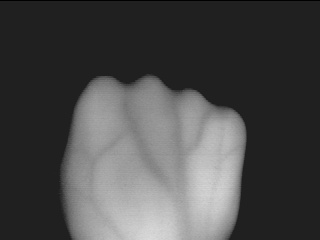
\includegraphics[width=0.4\paperwidth]{optimal-thresholding/global/hand-original-image.jpg}
\caption{Original image of interest (\textit{0019hv3.bmp}) }
\label{fig:hand-original-image}
\end{figure}


\begin{figure}[h!]

\includegraphics[width=0.4\paperwidth]{optimal-thresholding/global/hand-global-threshold.jpg}
\centering
\caption{Global thresholded image [optimal] (\textit{Threshold = 95.51}) }
\label{fig:hand-global-threshold}
\end{figure}



\begin{figure}[h!]
\centering
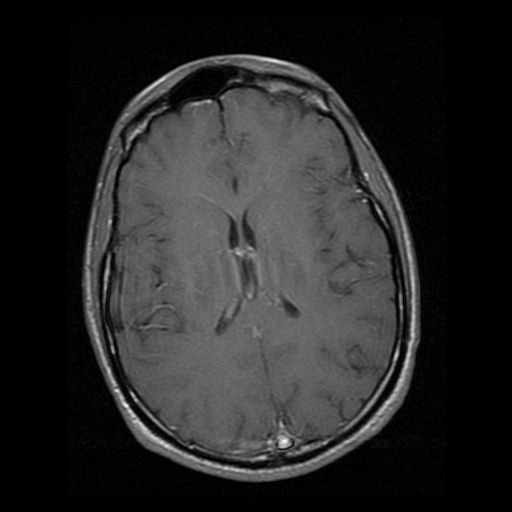
\includegraphics[width=0.4\paperwidth]{optimal-thresholding/global/MRI-original-image.jpg}
\caption{Original image of interest (\textit{MR1Brain2.jpg}) }
\label{fig:MRI-original-image}
\end{figure}


\begin{figure}[h!]
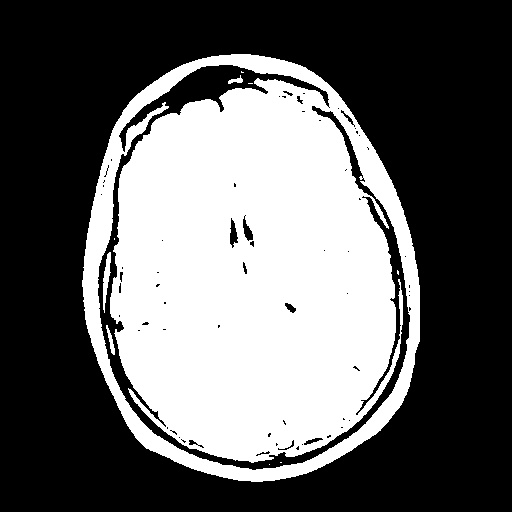
\includegraphics[width=0.4\paperwidth]{optimal-thresholding/global/MRI-global-threshold.jpg}
\centering
\caption{Global thresholded image [optimal] (\textit{Threshold = 48.49}) }
\label{fig:MRI-global-threshold}
\end{figure}


\section*{Local Optimal Thresholding: Implementation}
Local optimal thresholding is based on dividing the images unit blocks and threshold each block
independently by optimal method then add all the thresholded blocks to get the output thresholded image.
 
The localOptimalThresholding function takes the input image to be thresholded using \textit{Optimal Thresholding} , block size returns the thresholded image.

\subsection*{\textbf{Results}}
Using our implementation of local optimal thresholding we could produce the following images. see Figure ~\ref{fig:MRI-original-image}, ~\ref{fig:MRI-local-threshold16},~\ref{fig:MRI-local-threshold32},  ~\ref{fig:MRI-local-threshold64},~\ref{fig:MRI-local-threshold128}, and ~\ref{fig:MRI-local-threshold256}. 

\begin{figure}[h!]
\centering
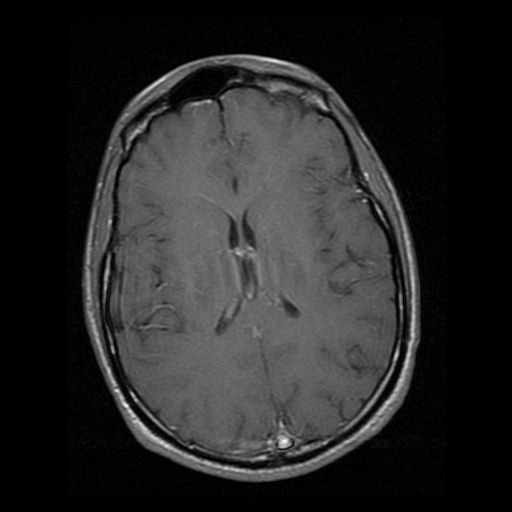
\includegraphics[width=0.4\paperwidth]{optimal-thresholding/global/MRI-original-image.jpg}
\caption{Original image of interest (\textit{MR1Brain2.jpg ( 512 X 512 )}) }
\label{fig:MRI-original-image}
\end{figure}


\begin{figure}[h!]
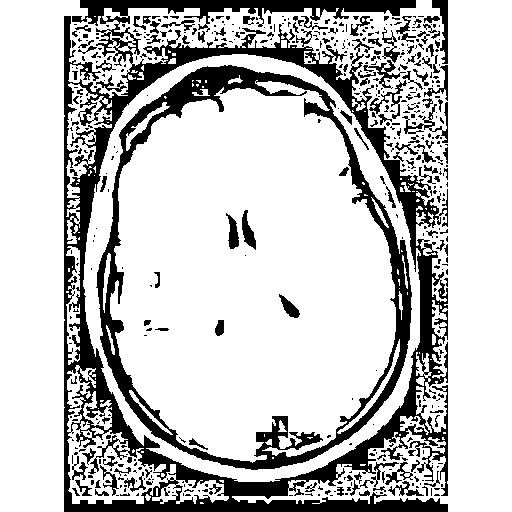
\includegraphics[width=0.4\paperwidth]{optimal-thresholding/local/MRI-local-threshold16.jpg}
\centering
\caption{local thresholded image [optimal] (\textit{Block size 16 }) }
\label{fig:MRI-local-threshold16}
\end{figure}


\begin{figure}[h!]
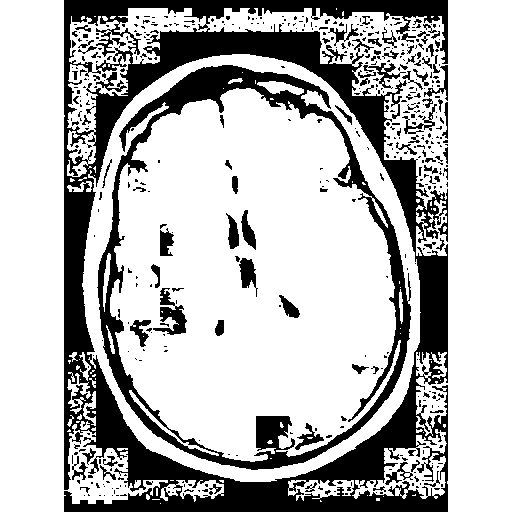
\includegraphics[width=0.4\paperwidth]{optimal-thresholding/local/MRI-local-threshold32.jpg}
\centering
\caption{local thresholded image [optimal] (\textit{Block size 32 }) }
\label{fig:MRI-local-threshold32}
\end{figure}


\begin{figure}[h!]
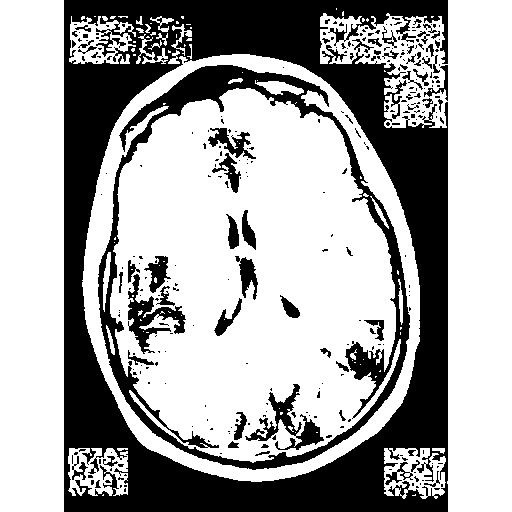
\includegraphics[width=0.4\paperwidth]{optimal-thresholding/local/MRI-local-threshold64.jpg}
\centering
\caption{local thresholded image [optimal] (\textit{Block size 64 }) }
\label{fig:MRI-local-threshold64}
\end{figure}


\begin{figure}[h!]
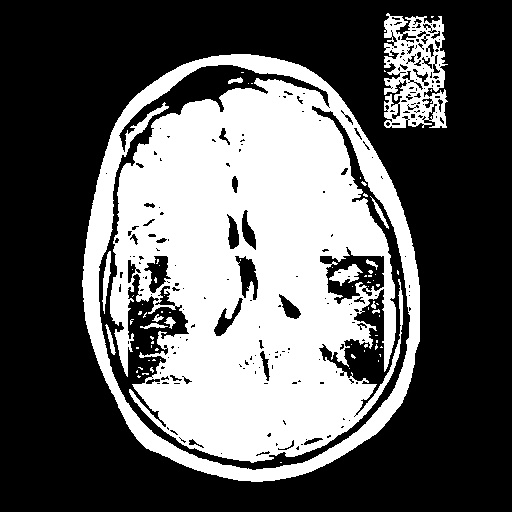
\includegraphics[width=0.4\paperwidth]{optimal-thresholding/local/MRI-local-threshold128.jpg}
\centering
\caption{local thresholded image [optimal] (\textit{Block size 128 }) }
\label{fig:MRI-local-threshold128}
\end{figure}
 

\begin{figure}[h!]
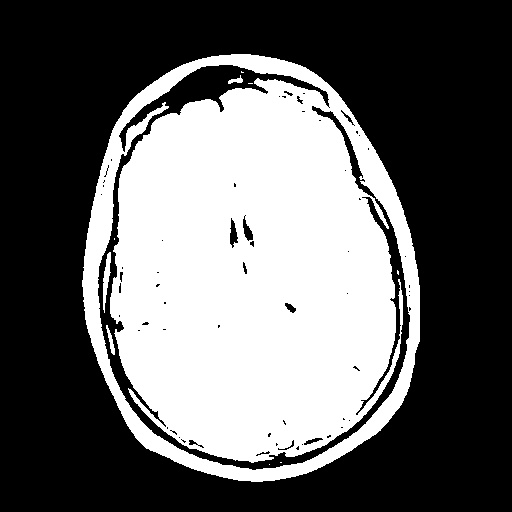
\includegraphics[width=0.4\paperwidth]{optimal-thresholding/local/MRI-local-threshold256.jpg}
\centering
\caption{local thresholded image [optimal] (\textit{Block size 256 }) }
\label{fig:MRI-local-threshold256}
\end{figure} 


\subsection*{Otsu Thresholding} 
The general overview of thresholding  using \textit{Otsu Thresholding}:
At each gray level(0:255) we do the following: 
\begin{enumerate}
\item Calculating background weight and foreground weight.
\item Calculating background mean and foreground mean.
\item Calculating between class variance as follows : 

\begin{equation} \label{betweenclassvaraince_eqn}
{W_f}{W_b}{{(meanf-meanb)}^2}
\end{equation}

\item Calculating maximum Between Class Variance (minimum within class variance). 
\end{enumerate} 

\textbf{The otsu threshold is the gray level corresponding to maximum Between Class Variance 		(Minimum Within Class Variance).}

\section*{Global Otsu Thresholding: Implementation}
The globalOtsuThresholding function takes the input image to be thresholded using \textit{Otsu Thresholding} and returns the thresholded image and otsu threshold.


\subsection*{\textbf{Results}}
Using our implementation of global otsu thresholding we could produce the following images. see Figure ~\ref{fig:Beads-original-image},~\ref{fig:Beads-global-threshold-otsu},~\ref{fig:MRI-original-image}, and ~\ref{fig:MRI-global-threshold-otsu}.


\begin{figure}[h!]
\centering
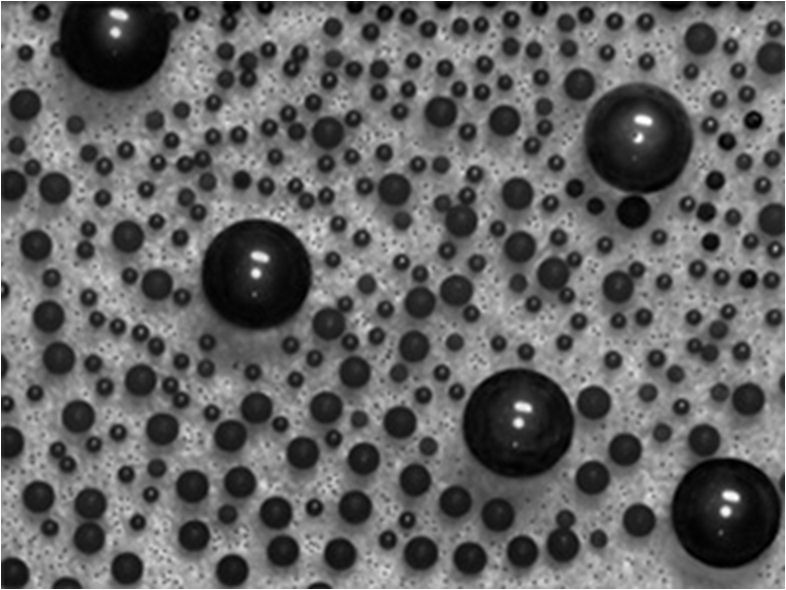
\includegraphics[width=0.4\paperwidth]{otsu-thresholding/global/Beads.jpg}
\caption{Original image of interest (\textit{Beads.jpg}) }
\label{fig:Beads-original-image}
\end{figure}


\begin{figure}[h!]
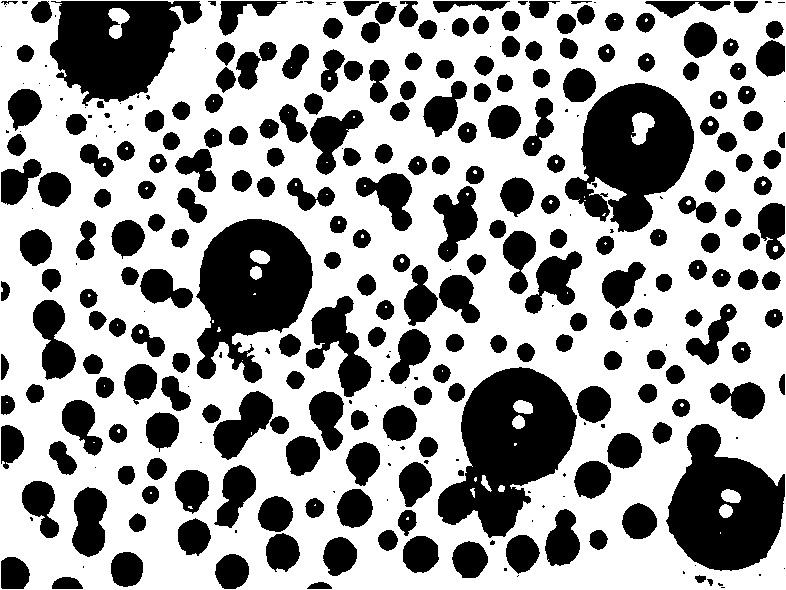
\includegraphics[width=0.4\paperwidth]{otsu-thresholding/global/Beads-global-otsu.jpg}
\centering
\caption{Global thresholded image [otsu]  (\textit{Threshold = 90}) }
\label{fig:Beads-global-threshold-otsu}
\end{figure}


\begin{figure}[h!]
\centering
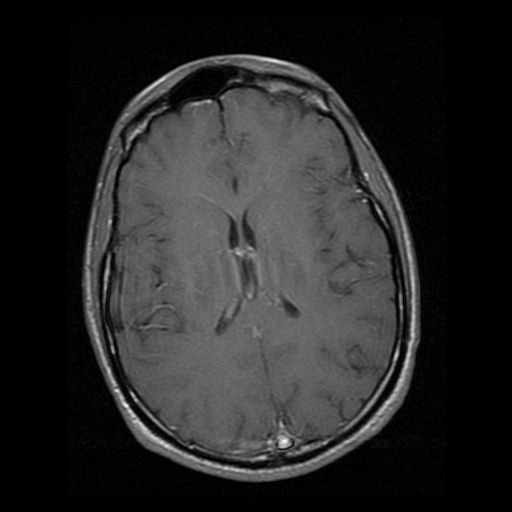
\includegraphics[width=0.4\paperwidth]{optimal-thresholding/global/MRI-original-image.jpg}
\caption{Original image of interest (\textit{MR1Brain2.jpg}) }
\label{fig:MRI-original-image}
\end{figure}


\begin{figure}[h!]
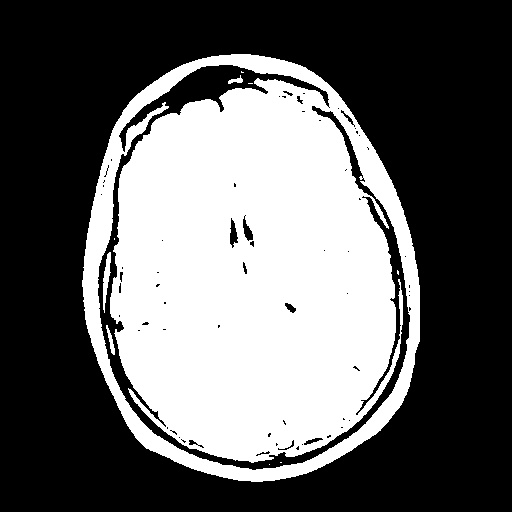
\includegraphics[width=0.4\paperwidth]{otsu-thresholding/global/MRI-global-threshold-otsu.jpg}
\centering
\caption{Global thresholded image [otsu]  (\textit{Threshold = 49}) }
\label{fig:MRI-global-threshold-otsu}
\end{figure}


\section*{Local Optimal Thresholding: Implementation}
Local Otsu thresholding is based on dividing the images unit blocks and threshold each block
independently by otsu method then add all the thresholded blocks to get the output thresholded image.
 
The localOptimalThresholding function takes the input image to be thresholded using \textit{Optimal Thresholding} , block size returns the thresholded image.

\subsection*{\textbf{Results}}
Using our implementation of local otsu thresholding we could produce the following images. see Figure ~\ref{fig:MRI-original-image}, ~\ref{fig:MRI-local-threshold-otsu16},~\ref{fig:MRI-local-threshold-otsu32},  ~\ref{fig:MRI-local-threshold-otsu64},~\ref{fig:MRI-local-threshold-otsu128}, and ~\ref{fig:MRI-local-threshold-otsu256}. 

\begin{figure}[h!]
\centering
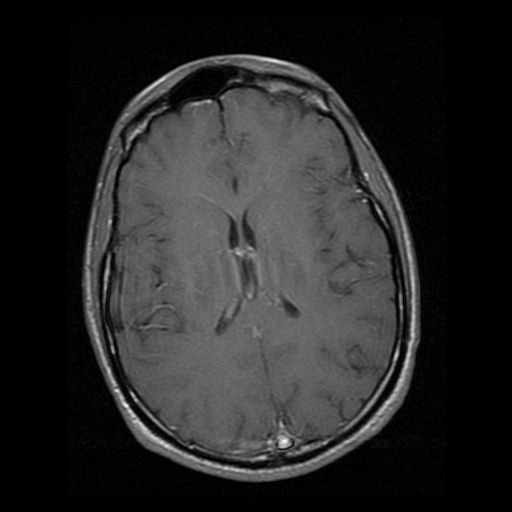
\includegraphics[width=0.4\paperwidth]{optimal-thresholding/global/MRI-original-image.jpg}
\caption{Original image of interest (\textit{MR1Brain2.jpg ( 512 X 512 )}) }
\label{fig:MRI-original-image}
\end{figure}


\begin{figure}[h!]
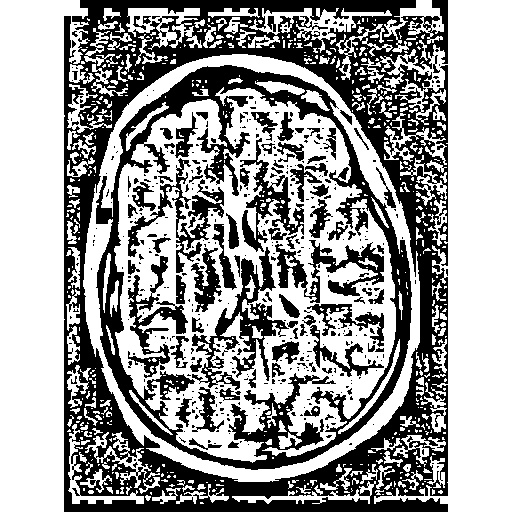
\includegraphics[width=0.4\paperwidth]{otsu-thresholding/local/MRI-local-threshold-otsu16.jpg}
\centering
\caption{local thresholded image [otsu] (\textit{Block size 16 }) }
\label{fig:MRI-local-threshold-otsu16}
\end{figure}


\begin{figure}[h!]
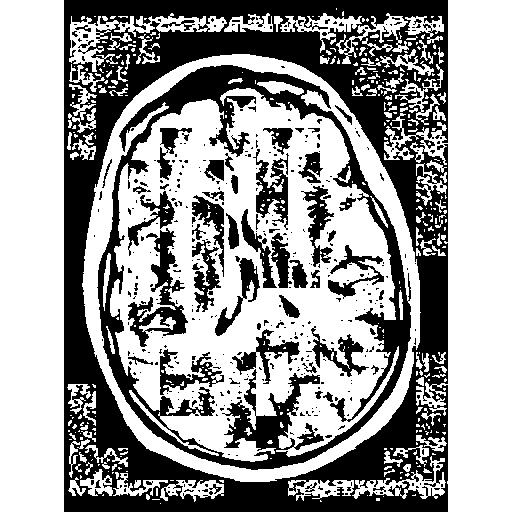
\includegraphics[width=0.4\paperwidth]{otsu-thresholding/local/MRI-local-threshold-otsu32.jpg}
\centering
\caption{local thresholded image [otsu] (\textit{Block size 32 }) }
\label{fig:MRI-local-threshold-otsu32}
\end{figure}


\begin{figure}[h!]
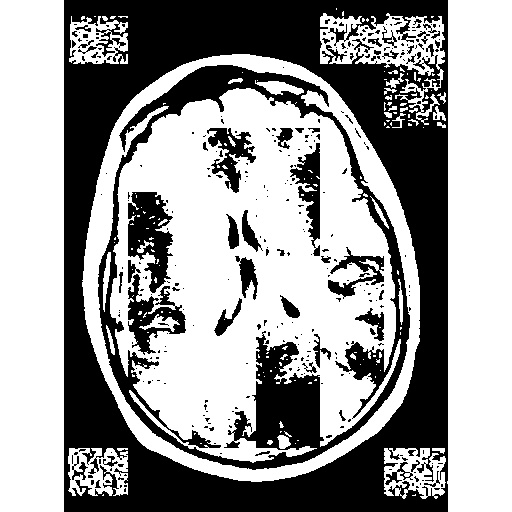
\includegraphics[width=0.4\paperwidth]{otsu-thresholding/local/MRI-local-threshold-otsu64.jpg}
\centering
\caption{local thresholded image [otsu] (\textit{Block size 64 }) }
\label{fig:MRI-local-threshold-otsu64}
\end{figure}


\begin{figure}[h!]
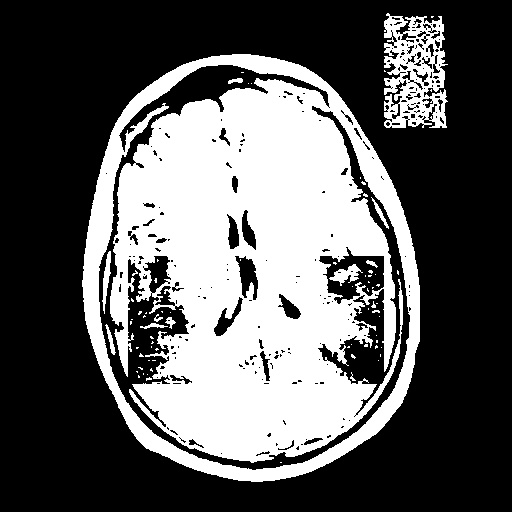
\includegraphics[width=0.4\paperwidth]{otsu-thresholding/local/MRI-local-threshold-otsu128.jpg}
\centering
\caption{local thresholded image [otsu] (\textit{Block size 128 }) }
\label{fig:MRI-local-threshold-otsu128}
\end{figure}
 

\begin{figure}[h!]
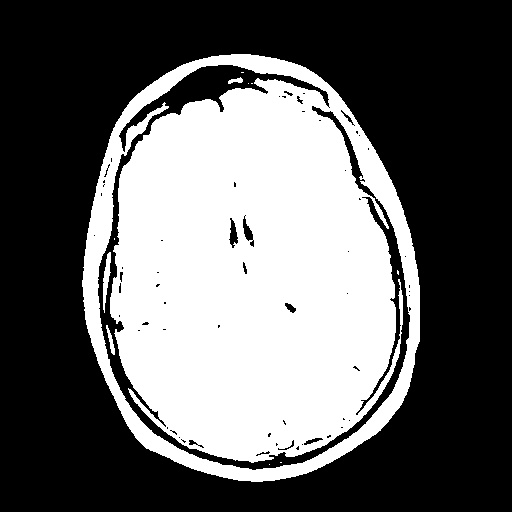
\includegraphics[width=0.4\paperwidth]{otsu-thresholding/local/MRI-local-threshold-otsu256.jpg}
\centering
\caption{local thresholded image [otsu] (\textit{Block size 256 }) }
\label{fig:MRI-local-threshold-otsu256}
\end{figure} 

\section{Part2: Segmentation}

\subsection*{K-means segmentation}
This type of segmentation is based on the traditional k-means clustering algorithm. In this k-means implementations, we cluster the image RGB components in the RGB color-space. \\
labels , centroids , wss = KmeansSegmentation( image , 4  )
\\
This function performs the kmeans in image for 4 clusters. It returns centroids, labels and the within-sum of squares


\subsubsection*{\textbf{Results}}  

Here are some of the results, in figure \ref{fig:Xray-kmean-4}
\begin{figure}[h!]
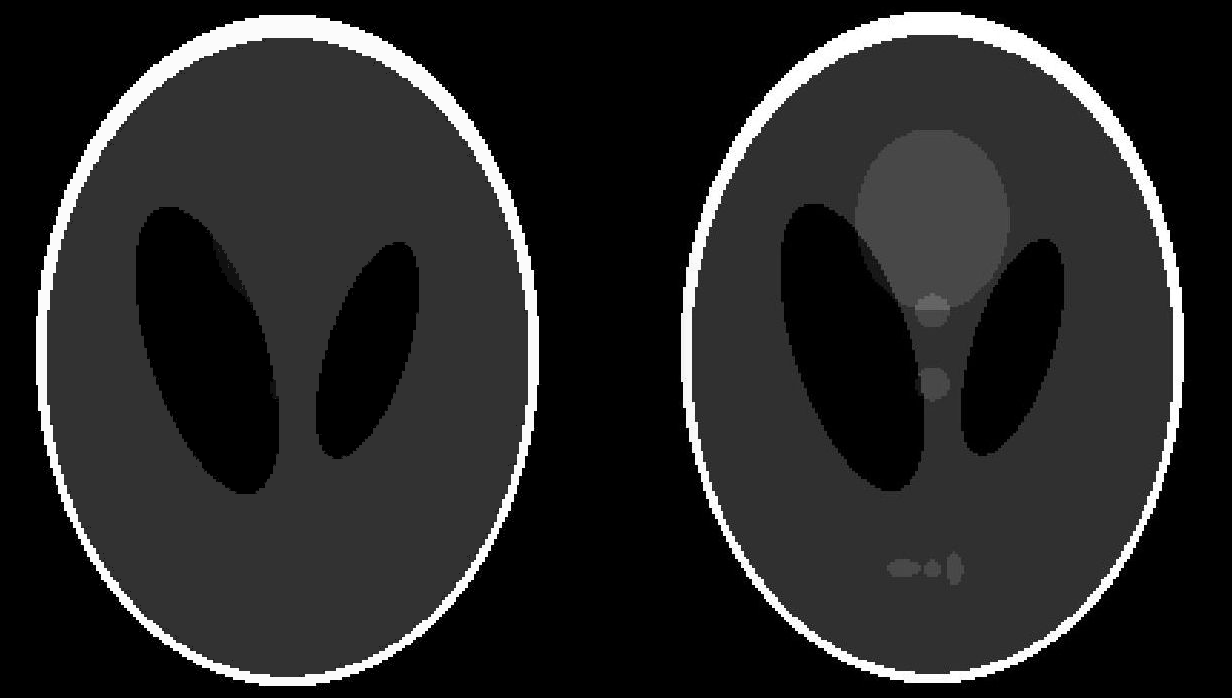
\includegraphics[width=0.4\paperwidth]{kmeans/kmean-4}
\centering
\caption{K-mean clustering to 4 clusters. The one on the right is the un-clustered, the other is th clustered one}
\label{fig:Xray-kmean-4}
\end{figure}

\subsection*{Regional Growing segmentation}
This type of segmentation is based on the Regional Growing segmentation algorithm. In this  implementations, we cluster the image RGB components in the RGB color-space. The colors used to identify regions are chosen randomly.\\

segmentedImage = RegionGrowingSegmentation(image)
\\
This function returns the segmented image of 'image'. The user select the region to be highlighted using the mouse pointer
\subsubsection*{textbf{Results}}  

Here are some of the results, in figure \ref{fig:regional-growing}
\begin{figure}[h!]
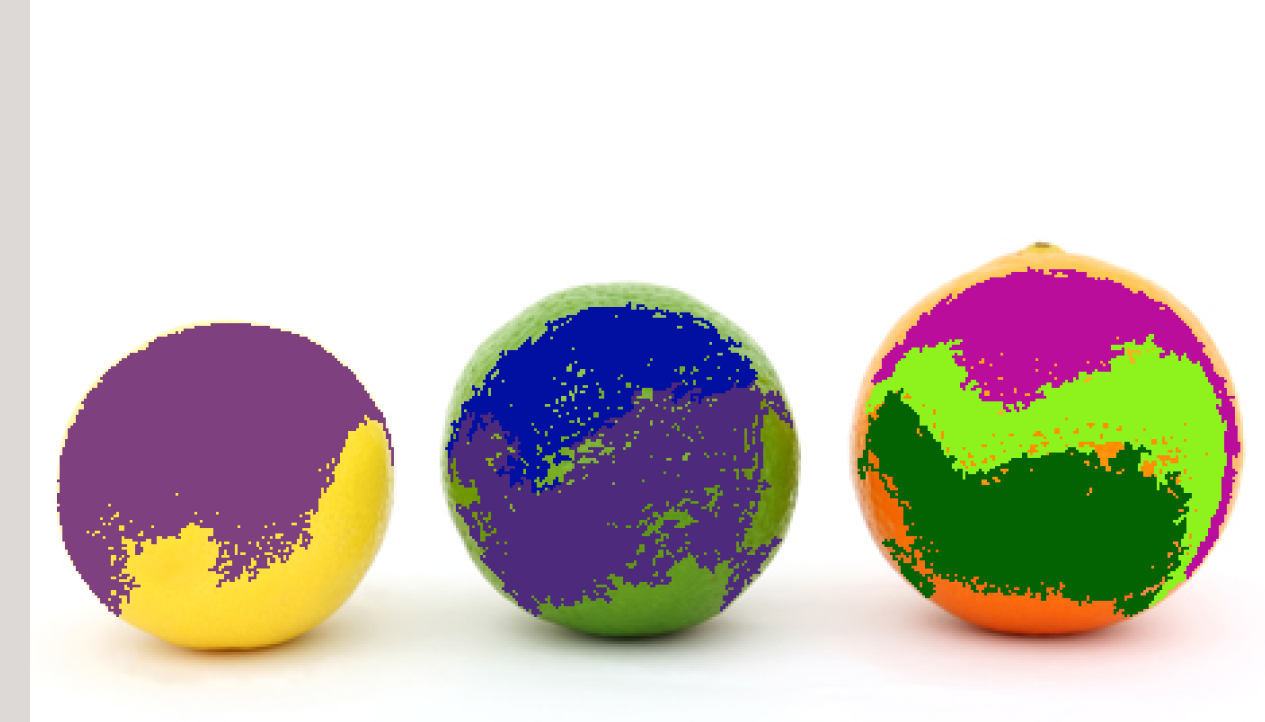
\includegraphics[width=0.4\paperwidth]{regional-growing/regional-growing}
\centering
\caption{Image is segmented using regional growing }
\label{fig:regional-growing}
\end{figure}

\subsection*{Mean Shift segmentation}
This type of segmentation is based on the Mean-shift segmentation algorithm. In this  implementations, we cluster the image RGB components in the UV color-space and the GB color-space.
\\
meanShift = meanShiftSeg( imageRGB, 7 )
\\This the instantiation of the mean-shift object, with the image either in RGB form or LUV. The other parameter is the window dim 
\\
segImage = meanShift.applyMeanShift()
\\The function applyShift(), perform the mean-shift on the clusters, then return the segmented image

\subsubsection*{\textbf{Results}}  

Here are some of the results, in figure \ref{fig:mean-shift-4}
\begin{figure}[h!]
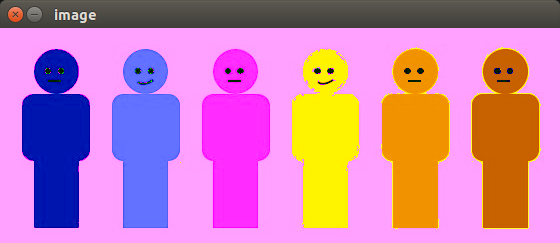
\includegraphics[width=0.4\paperwidth]{mean-shift/window128-4cluster}
\centering
\caption{Image is segmented using mean-shift , 4 clusters, UV color-space }
\label{fig:mean-shift-4}
\end{figure}

\begin{figure}[h!]
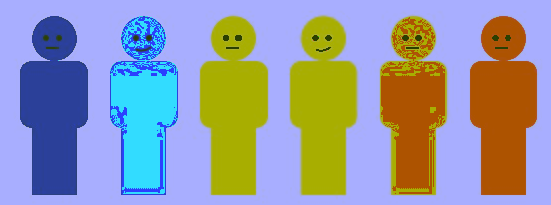
\includegraphics[width=0.4\paperwidth]{mean-shift/mean-shift-rgb-4}
\centering
\caption{Image is segmented using mean-shift , 4 clusters, GB color-space }
\label{fig:mean-shift-4}
\end{figure}

\begin{figure}[H]
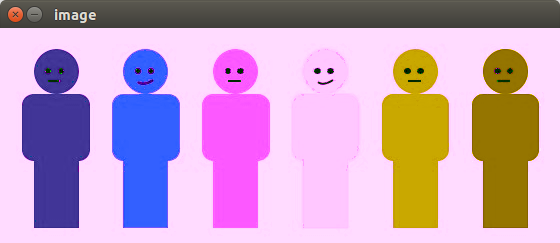
\includegraphics[width=0.4\paperwidth]{mean-shift/window32-64cluster}
\centering
\caption{Image is segmented using mean-shift, 64 clusters, LUV color-space }
\label{fig:mean-shift-64}
\end{figure}


\end{document}

